\documentclass[10pt,usenames,dvipsnames]{beamer}

\usetheme[progressbar=frametitle]{metropolis}
\usepackage{graphicx}
\usepackage{caption}
\usepackage{appendixnumberbeamer}

\usepackage{booktabs}
\usepackage[scale=2]{ccicons}

\usepackage{pgfplots}
\usepackage{tikz}
\usepgfplotslibrary{dateplot}
\usepackage{xspace}
\newcommand{\themename}{\textbf{\textsc{metropolis}}\xspace}
\usepackage{biblatex}
\bibliography{presentation}
\usepackage{listings}
\usepackage{minted}
\usepackage{verbatim}
\def\b#1{\mathbf{ #1}}
\title{Automatic Synthesis of Low Complexity Translation Operators for the Fast Multipole Method}
\author{\textbf{Isuru Fernando}, Andreas Kl{\"o}ckner}
% \titlegraphic{\hfill\includegraphics[height=1.5cm]{logo.pdf}}
\usepackage{array}
\newcolumntype{L}{>{\centering\arraybackslash}m{3cm}}
\begin{document}

\maketitle

\begin{frame}[fragile]{Outline}
 \begin{itemize}
  \item Quick introduction to Taylor series based Fast Multipole Method
  \item Compressed Taylor Series based expansions and translations
  \item Results - accuracy and time complexity
 \end{itemize}

\end{frame}

\begin{frame}[fragile]{N-body problem}
Let $(\b s_j)_{j=1}^{n}$ be sources and $(\b t_i)_{i=1}^{n}$ be targets. Potential at target $\b t_i$ is the sum of all potentials from the sources $\b s_j$ given by,
\[\sum_{j} \psi(\b t_i, \b s_j).\]
For example, \[\psi(\b t_i, \b s_j) = \frac{1}{\text{dist}(\b t_i, \b s_j)}.\]
\begin{center}
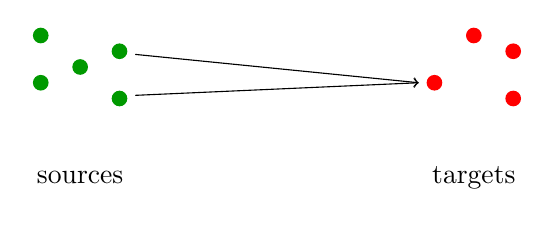
\begin{tikzpicture}[x=1cm,y=0.4cm]
\foreach \Point in {(-2,1.5), (-1,1), (-1.5, 2), (-2,3), (-1,2.5)}{
    \draw \Point node[anchor=center,fill=black!40!green,circle,scale=0.6] {};
}

\foreach \Point in {(3,1.5), (4,1), (3.5,3), (4,2.5)}{
    \draw \Point node[anchor=center,fill=red,circle,scale=0.6] {};
}
\node at (-1.5,-1.5) {sources};
\node at (3.5,-1.5) {targets};

\draw[->] (-0.8,1.1) -- (2.8,1.5);
\draw[->] (-0.8,2.4) -- (2.8,1.5);
\end{tikzpicture}
\end{center}

$n$ sources and $n$ targets $\implies$  $\mathcal{O}(n^2)$ cost.

\end{frame}

\begin{frame}[fragile]{Fast Multipole Method}

Algorithm by Greengard and Rokhlin (1987) to compute the potentials in $\mathcal{O}(n)$ time.
\begin{figure}
\includegraphics[scale=0.15]{figures/quadtree.png}
\caption{Carrier et al, 1988}
\end{figure}
Useful for solving PDE BVPs with Integral equation methods via layer potentials.
\[
    \int_{\Gamma} G(x - y) \sigma_y dy.
\]
\end{frame}

%\begin{frame}[fragile]{Multipole Expansion}
%
%\begin{center}
%\begin{tikzpicture}[x=1cm,y=0.4cm]
%
%
%\foreach \Point in {(0.25,0), (1, 1), (0.5, 0.75), (0.75, 0.25), (0.5, -0.25), (0.9, -0.25)}{
%    \draw \Point node[anchor=center,fill=black!40!green,circle,scale=0.6] {};
%}
%
%\foreach \Point in {(0.25,3), (1.0, 3.5), (0.25, 3.4), (0.85, 3.2), (0.5, 2.5), (0.9, 2.5)}{
%    \draw \Point node[anchor=center,fill=black!40!green,circle,scale=0.6] {};
%}
%
%\foreach \Point in {(0.25,5), (1.0, 5.5), (0.5, 5.4), (0.85, 5.2), (0.5, 5.5), (0.2, 4.5),(0.7, 4.3)}{
%    \draw \Point node[anchor=center,fill=red,circle,scale=0.6] {};
%}
%
%\foreach \Point in {(3.25,3), (3.0, 3.7), (3.3, 3.2), (3.65, 3.4), (3.7, 3.7), (3.2, 2.5),(3.9, 2.3)}{
%    \draw \Point node[anchor=center,fill=red,circle,scale=0.6] {};
%}
%
%%\draw (0.2, 0) circle (1.1cm) node[above] {$\boldsymbol{c}_0$};
%%\draw (2.7, 0) circle (1.1cm) node[above] {$\boldsymbol{c}_1$};
%%\draw (1.45, 0) circle (2.35cm) node[above] {$\boldsymbol{c}$};
%
%\end{tikzpicture}
%\end{center}
%\end{frame}
%
%\begin{frame}[fragile]{Multipole Expansion}
%
%\begin{center}
%\begin{tikzpicture}[x=1cm,y=0.4cm]
%
%
%\foreach \Point in {(0.25,0), (1, 1), (0.5, 0.75), (0.75, 0.25), (0.5, -0.25), (0.9, -0.25)}{
%    \draw \Point node[anchor=center,fill=black!40!green,circle,scale=0.6] {};
%}
%
%\foreach \Point in {(0.25,3), (1.0, 3.5), (0.25, 3.4), (0.85, 3.2), (0.5, 2.5), (0.9, 2.5)}{
%    \draw \Point node[anchor=center,fill=black!40!green,circle,scale=0.6] {};
%}
%
%\foreach \Point in {(0.25,5), (1.0, 5.5), (0.5, 5.4), (0.85, 5.2), (0.5, 5.5), (0.2, 4.5),(0.7, 4.3)}{
%    \draw \Point node[anchor=center,fill=red,circle,scale=0.6] {};
%}
%
%\foreach \Point in {(3.25,3), (3.0, 3.7), (3.3, 3.2), (3.65, 3.4), (3.7, 3.7), (3.2, 2.5),(3.9, 2.3)}{
%    \draw \Point node[anchor=center,fill=red,circle,scale=0.6] {};
%}
%
%\draw[->, thick] (0,0) to [bend left] node[left] {multipole} (0,5);
%\draw[->, thick] (1.2,2.5) to [bend right] node[right] {direct} (1.2,5);
%%\draw (0.2, 0) circle (1.1cm) node[above] {$\boldsymbol{c}_0$};
%%\draw (2.7, 0) circle (1.1cm) node[above] {$\boldsymbol{c}_1$};
%\draw (0.7, 0.2) circle (0.6cm) node[above,fill=black,circle,scale=0.3,label=$\boldsymbol{c_1}$] {};
%
%\end{tikzpicture}
%\end{center}
%\end{frame}
%
%\begin{frame}[fragile]{Multipole Translation}
%
%\begin{center}
%\begin{tikzpicture}[x=1cm,y=0.4cm]
%
%
%\foreach \Point in {(0.25,0), (1, 1), (0.5, 0.75), (0.75, 0.25), (0.5, -0.25), (0.9, -0.25)}{
%    \draw \Point node[anchor=center,fill=black!40!green,circle,scale=0.6] {};
%}
%
%\foreach \Point in {(0.25,3), (1.0, 3.5), (0.25, 3.4), (0.85, 3.2), (0.5, 2.5), (0.9, 2.5)}{
%    \draw \Point node[anchor=center,fill=black!40!green,circle,scale=0.6] {};
%}
%
%\foreach \Point in {(0.25,5), (1.0, 5.5), (0.5, 5.4), (0.85, 5.2), (0.5, 5.5), (0.2, 4.5),(0.7, 4.3)}{
%    \draw \Point node[anchor=center,fill=red,circle,scale=0.6] {};
%}
%
%\foreach \Point in {(3.25,3), (3.0, 3.7), (3.3, 3.2), (3.65, 3.4), (3.7, 3.7), (3.2, 2.5),(3.9, 2.3)}{
%    \draw \Point node[anchor=center,fill=red,circle,scale=0.6] {};
%}
%
%\draw[->, thick] (0.7,0.2) to [bend left] node[left] {} (0.7,1.35);
%\draw[->, thick] (1.8,1.9) -- node[below] {} (3,3);
%%\draw (0.2, 0) circle (1.1cm) node[above] {$\boldsymbol{c}_0$};
%%\draw (2.7, 0) circle (1.1cm) node[above] {$\boldsymbol{c}_1$};
%\draw (0.7, 0.2) circle (0.6cm) node[above,fill=black,circle,scale=0.3,label=south:$\boldsymbol{c_1}$] {};
%\draw (0.7, 1.35) circle (1.1cm) node[above,fill=black,circle,scale=0.3,label=$\boldsymbol{c_2}$] {};
%
%\end{tikzpicture}
%\end{center}
%
%Multipole expansion around center $\b c_2$.
%\end{frame}


 \begin{frame}[fragile]{Taylor Series based FMM}
 
 Local expansion:
 \[
  \psi(\b t, \b s) = \sum_{|m| \le k} \underbrace{\frac{D_{\b t}^m \psi(\b t, \b s)\Bigr|_{\b t = \b c}}{m!}}_{\text{depends on src/ctr}} \underbrace{(\b t - \b       c)^m}_{\text{depends on tgt/ctr}}
 \]
 
 Multipole expansion:
 \[
  \psi(\b t, \b s) = \sum_{|m| \le k} \underbrace{\frac{D_{\b s}^m \psi(\b t, \b s)\Bigr|_{\b s = \b c}}{m!}}_{\text{depends on tgt/ctr}} \underbrace{(\b s - \b       c)^m}_{\text{depends on src/ctr}}
 \]
 \end{frame}

\begin{frame}[fragile]{Taylor Series based FMM}

 Some Expansion Types:
 \begin{itemize}
     \item Expansions using separation of angular variables (Spherical harmonics, Fourier-bessel based)
     \item Linear Algebra (Eg: Kernel-independent FMM)
     \item Taylor series based (Cartesian) expansions
 \end{itemize}

\renewcommand{\arraystretch}{2}

 \begin{table}[]
 \scriptsize
 \begin{tabular}{l|l}
     Pros & Cons \\ \hline
     - Easily tractable symbolically & - Expansions $\mathrm{O}(p^3)$ compared to $\mathrm{O}(p^2)$ \\
     \hspace{1 mm} for any kernel & - Translations $\mathrm{O}(p^6)$ compared to $\mathrm{O}(p^2\log(p))$ \\
    & - Stability issues \\
 \end{tabular}
     \caption{Pros and cons of Taylor series based expansions}
 \end{table}

\end{frame}
\begin{frame}[fragile]{Taylor Series based FMM}
  Goals:
    \begin{itemize}
        \item Find a way to reduce Taylor series cost.
        \item Use the Taylor series to automate FMM for "any" kernel
    \end{itemize}
\end{frame}

\begin{frame}[fragile]{Compressed Multipole Expansion}
 When $\psi$ satisfies the Helmholtz equation,
 \[
  \psi_{x x} + \psi_{y y} + \kappa^2 \psi = 0.
 \]

 Recall
 \[
 \psi(\b t, \b s) = \sum_{|m| \le p} \underbrace{\frac{D_{\b s}^m \psi(\b t, \b s)\Bigr|_{\b s = \b c}}{m!}}_{\text{depends on tgt/ctr}} \underbrace{(\b s - \b c)^m}_{\text{depends on src/ctr}}.
 \]
 From the PDE we have
 \begin{align*}
  c_1 \psi_{x x} +  c_2 \psi_{y y} + c_3 \psi 
  &= c_1 \psi_{x x} +  c_2 (-\psi_{x x} - \kappa^2 \psi) + c_3 \psi \\
  &= (c_1 - c_2) \psi_{x x} + 0 \psi_{y y} +\psi (c_3 - \kappa^2 c_2).
 \end{align*}
\end{frame}



\begin{frame}[fragile]{Compressed Multipole Expansion}
 
 For Helmholtz equation we also have
 \[
     \psi_{x x y y} + \psi_{y y y y}  + \kappa^2 \psi_{y y} = 0,
 \]
 \[
     \psi_{x x x x} + \psi_{x x y y}  + \kappa^2 \psi_{x x} = 0.
 \]
\begin{center}
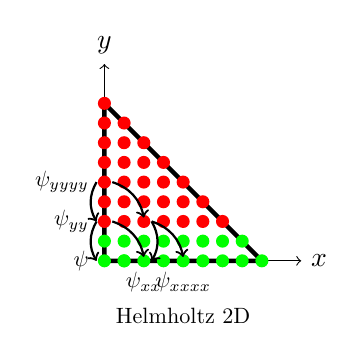
\begin{tikzpicture}[scale=0.5]
\draw[->] (0,0)--(5,0) node[right]{$x$};
\draw[->] (0,0)--(0,5) node[above]{$y$};
\draw[ultra thick] (0,0) node[anchor=north]{}
  -- (4,0) node[anchor=north]{}
  -- (0,4) node[anchor=south]{}
  -- cycle;
  
\foreach \Point in { (0, 0), (0.5, 0), (1.0, 0), (1.5, 0), (2.0, 0), (2.5, 0), (3.0, 0), (3.5, 0), (4.0, 0), (0.5, 0), (0, 0.5), (0.5, 0.5), (1.0, 0.5), (1.5, 0.5), (2.0, 0.5), (2.5, 0.5), (3.0, 0.5), (3.5, 0.5)}{
    \draw \Point node[anchor=center,fill=green,circle,scale=0.5] {};
}

\foreach \Point in { (0.0, 1.0), (0.0, 1.5), (0.0, 2.0), (0.0, 2.5), (0.0, 3.0), (0.0, 3.5), (0.0, 4.0), (0.5, 1.0), (0.5, 1.5), (0.5, 2.0), (0.5, 2.5), (0.5, 3.0), (0.5, 3.5), (1.0, 1.0), (1.0, 1.5), (1.0, 2.0), (1.0, 2.5), (1.0, 3.0), (1.5, 1.0), (1.5, 1.5), (1.5, 2.0), (1.5, 2.5), (2.0, 1.0), (2.0, 1.5), (2.0, 2.0), (2.5, 1.0), (2.5, 1.5), (3.0, 1.0) }{
    \draw \Point node[anchor=center,fill=red,circle,scale=0.5] {};
}

\draw[->, thick] (-0.2,2) to [bend right] node[right] {} (-0.2,1);
\draw[->, thick] (0.2,2) to [bend left] node[right] {} (1,1.1);
\draw[->, thick] (0.2,1) to [bend left] node[right] {} (1,0.1);
\draw[->, thick] (1.2,1) to [bend left] node[right] {} (2,0.1);
\draw[->, thick] (-0.2,1) to [bend right] node[right] {} (-0.2,0);
\draw[->, thick] (1.2,1) to [bend left] node[left] {} (1.2,0);


\node[left,scale=0.8] at (-0.2,0) {$\psi$};
\node[left,scale=0.8] at (-0.2,1) {$\psi_{y y}$};
\node[left,scale=0.8] at (-0.2,2) {$\psi_{y y y y}$};

\node[below,scale=0.8] at (1,-0.1) {$\psi_{x x}$};
\node[below,scale=0.8] at (2,-0.1) {$\psi_{x x x x}$};

\node[below,scale=0.8] at (2,-1) {Helmholtz 2D};

\end{tikzpicture}
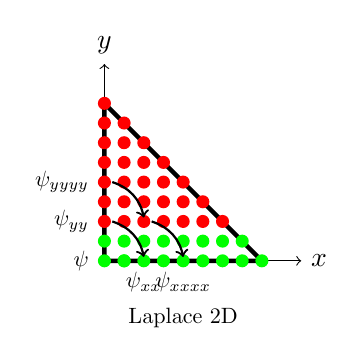
\begin{tikzpicture}[scale=0.5]
\draw[->] (0,0)--(5,0) node[right]{$x$};
\draw[->] (0,0)--(0,5) node[above]{$y$};
\draw[ultra thick] (0,0) node[anchor=north]{}
  -- (4,0) node[anchor=north]{}
  -- (0,4) node[anchor=south]{}
  -- cycle;
  
\foreach \Point in { (0, 0), (0.5, 0), (1.0, 0), (1.5, 0), (2.0, 0), (2.5, 0), (3.0, 0), (3.5, 0), (4.0, 0), (0.5, 0), (0, 0.5), (0.5, 0.5), (1.0, 0.5), (1.5, 0.5), (2.0, 0.5), (2.5, 0.5), (3.0, 0.5), (3.5, 0.5)}{
    \draw \Point node[anchor=center,fill=green,circle,scale=0.5] {};
}

\foreach \Point in { (0.0, 1.0), (0.0, 1.5), (0.0, 2.0), (0.0, 2.5), (0.0, 3.0), (0.0, 3.5), (0.0, 4.0), (0.5, 1.0), (0.5, 1.5), (0.5, 2.0), (0.5, 2.5), (0.5, 3.0), (0.5, 3.5), (1.0, 1.0), (1.0, 1.5), (1.0, 2.0), (1.0, 2.5), (1.0, 3.0), (1.5, 1.0), (1.5, 1.5), (1.5, 2.0), (1.5, 2.5), (2.0, 1.0), (2.0, 1.5), (2.0, 2.0), (2.5, 1.0), (2.5, 1.5), (3.0, 1.0) }{
    \draw \Point node[anchor=center,fill=red,circle,scale=0.5] {};
}

\draw[->, thick] (0.2,2) to [bend left] node[right] {} (1,1.1);
\draw[->, thick] (0.2,1) to [bend left] node[right] {} (1,0.1);
\draw[->, thick] (1.2,1) to [bend left] node[right] {} (2,0.1);

\node[left,scale=0.8] at (-0.2,0) {$\psi$};
\node[left,scale=0.8] at (-0.2,1) {$\psi_{y y}$};
\node[left,scale=0.8] at (-0.2,2) {$\psi_{y y y y}$};

\node[below,scale=0.8] at (1,-0.1) {$\psi_{x x}$};
\node[below,scale=0.8] at (2,-0.1) {$\psi_{x x x x}$};
\node[below,scale=0.8] at (2,-1) {Laplace 2D};

\end{tikzpicture}
\end{center}

All the coefficients represented by red dots get lumped into "green" coefficients.

Count of expansion coefficients goes from $\mathcal{O}(p^d)$ to $\mathcal{O}(p^{d-1})$.

\end{frame}



\begin{frame}[fragile]{Compressed Local Expansion}

Recall
\[
 \psi(\b t, \b s) = \sum_{|m| \le p} \underbrace{\frac{D_{\b t}^m \psi(\b t, \b s)\Bigr|_{\b t = \b c}}{m!}}_{\text{depends on src/ctr}} \underbrace{(\b t - \b c)^m}_{\text{depends on tgt/ctr}}
\]

Out of $\mathcal{O}(p^d)$ coefficients, only $\mathcal{O}(p^{d-1})$ are independent.

This makes the number of terms of a local expansion $\mathcal{O}(p^{d-1})$.
 
\end{frame}

\begin{frame}[fragile]{Calculating derivatives for Local Expansion}

Tausch (2003) proposes an algorithm which has an amortized $\mathcal{O}(p)$ time
assuming that the Green's function is radially symmetric.

We found several formulae to calculate these in amortized $\mathcal{O}(1)$ time.

For Laplace 3D
\tiny
\begin{align*}
    r^2 \frac{\partial^{n+m+l}}{\partial x^{n} y^m z^l} \left(\frac{1}{r}\right) =
              & -(2n-1)x \frac{\partial^{n+m-1}}{\partial x^{n-1} y^m z^l} \left(\frac{1}{r}\right)
              - (n-1)^2 \frac{\partial^{n+m-2}}{\partial x^{n-2}y^m z^l} \left(\frac{1}{r}\right)
              - 2m y \frac{\partial^{n+m-1}}{\partial x^{n} y^{m-1} z^l} \left(\frac{1}{r}\right) \\
              &- m(m-1) \frac{\partial^{n+m-2}}{\partial x^{n} y^{m-2} z^l} \left(\frac{1}{r}\right)
              - 2l z \frac{\partial^{n+m-1}}{\partial x^{n} y^{m} z^{l-1}} \left(\frac{1}{r}\right)
              - l(l-1) \frac{\partial^{n+m-2}}{\partial x^{n} y^{m} z^{l-2}} \left(\frac{1}{r}\right)
\end{align*}.

\normalsize
For Biharmonic 2D,
\tiny
\begin{align*}
    r^2 \frac{\partial^{n+m}}{\partial x^{n}y^m} \left(r^2 \log(r)\right) = &
               -2(n-2)x \frac{\partial^{n+m-1}}{\partial x^{n-1}y^m} \left(r^2 \log(r)\right)
               -(n-1)(n-4) \frac{\partial^{n+m-2}}{\partial x^{n-2}y^m} \left(r^2 \log(r)\right) \\
               &-2 m y\frac{\partial^{n+m-1}}{\partial x^{n}y^{m-1}} \left(r^2 \log(r)\right)
               -m(m-1) \frac{\partial^{n+m-2}}{\partial x^{n}y^{m-2}} \left(r^2 \log(r)\right).
\end{align*}
\normalsize
This reduces the cost of P2L from $\mathcal{O}(p^d)$ to $\mathcal{O}(p^{d-1})$.

\end{frame}

\begin{frame}[fragile]{Naive Multipole Translation}
Let $c_1$ be the old center and $c$ be the new center. Then,
\begin{align*}
(\b s-\b c)^k &= \left(\left(\b s-\b c_1\right) + \left(\b c_1-\b c\right)\right)^k   \\
&= \sum_{l \le k} \binom{k}{l}\left(\b s-\b c_1\right)^l \left(\b c_1-\b c\right)^{k-l} \\
&= \sum_{l \le k} \beta_{k, l}\left(\b s-\b c_1\right)^l
\end{align*}

Cost: $\mathcal{O}(p^{2d})$.

\end{frame}

\begin{frame}[fragile]{Compressed Multipole Translation}

\begin{center}
\vspace*{-2mm}
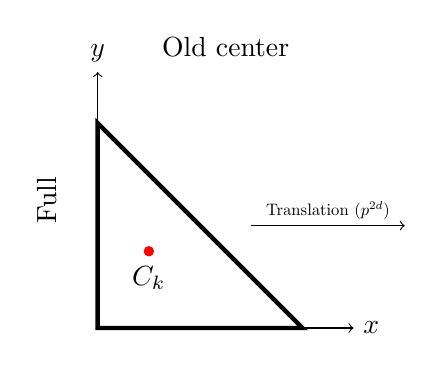
\begin{tikzpicture}[scale=0.65]

\node at (2.5,5.5) {Old center};
\node[rotate=90] at (-1,2.5) {Full};
\draw[->] (0,0)--(5,0) node[right]{$x$};
\draw[->] (0,0)--(0,5) node[above]{$y$};
\draw[ultra thick] (0,0) node[anchor=north]{}
  -- (4,0) node[anchor=north]{}
  -- (0,4) node[anchor=south]{}
  -- cycle;
\draw (1,1.5) node[anchor=center,fill=red,circle,scale=0.4,label=below:$C_k$] {};
\draw[->] (3, 2)-- node[above,scale=0.6]{Translation ($p^{2d}$)} (6,2);
\end{tikzpicture}
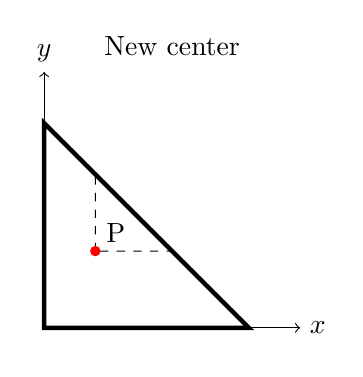
\begin{tikzpicture}[scale=0.65]
\node at (2.5,5.5) {New center};
\draw[->] (0,0)--(5,0) node[right]{$x$};
\draw[->] (0,0)--(0,5) node[above]{$y$};
\draw[ultra thick] (0,0) node[anchor=north]{}
  -- (4,0) node[anchor=north]{}
  -- (0,4) node[anchor=south]{}
  -- cycle;
\draw [dashed] (1,1.5) node[anchor=west]{}
  -- (1,3) node[anchor=north]{}
  -- (2.5,1.5) node[anchor=south]{}
  -- cycle;

\draw (1,1.5) node[anchor=center,fill=red,circle,scale=0.4] {};
\node[color=black] at (1.4,1.85) {P};
%\draw[->] (1,1.5)--(1.4,1.7) node[above]{};
%\draw [dashed,fill=gray] (1.5,1.8) node[fill=black,circle,anchor=center,scale=0.4,label=north:$T_{k+l}$]{};
\end{tikzpicture}

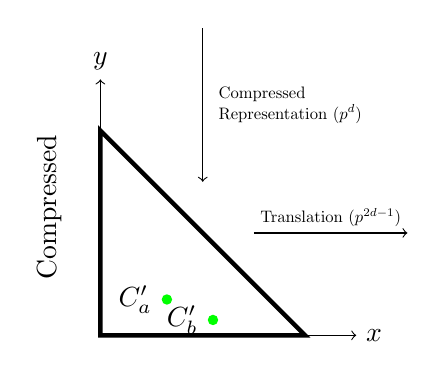
\begin{tikzpicture}[scale=0.65]
\node[rotate=90] at (-1,2.5) {Compressed};
\draw[->] (0,0)--(5,0) node[right]{$x$};
\draw[->] (0,0)--(0,5) node[above]{$y$};
\draw[ultra thick] (0,0) node[anchor=north]{}
  -- (4,0) node[anchor=north]{}
  -- (0,4) node[anchor=south]{}
  -- cycle;
\draw [dashed,fill=gray] (1.3,0.7) node[fill=green,circle,anchor=center,scale=0.4,label=west:$C'_{a}$]{};
\draw [dashed,fill=gray] (2.2,0.3) node[fill=green,circle,anchor=center,scale=0.4,label=west:$C'_{b}$]{};
\draw[->] (3, 2)-- node[above,scale=0.6]{Translation ($p^{2d-1}$)} (6,2);
\draw[->] (2, 6)-- node[right,scale=0.6]{\begin{tabular}{l} Compressed \\ Representation ($p^{d}$) \end{tabular}} (2,3);
\end{tikzpicture}
\begin{tikzpicture}[scale=0.65]
\draw[->] (0,0)--(5,0) node[right]{$x$};
\draw[->] (0,0)--(0,5) node[above]{$y$};
\draw[ultra thick] (0,0) node[anchor=north]{}
  -- (4,0) node[anchor=north]{}
  -- (0,4) node[anchor=south]{}
  -- cycle;
\draw [dashed,color=blue] (1.3,0.7) node[anchor=west]{}
  -- (1.3,2.7) node[anchor=north]{}
  -- (3.3,0.7) node[anchor=south]{}
  -- cycle;
\draw [dashed,color=orange] (2.2,0.3) node[anchor=west]{}
  -- (3.7,0.3) node[anchor=north]{}
  -- (2.2,1.8) node[anchor=south]{}
  -- cycle;
\draw [dashed,fill=gray] (1.3,0.7) node {};
\draw [dashed,fill=gray] (2.2,0.3) node {};

\draw [dashed,fill=gray] (1.3,0.7) node[fill=green,circle,anchor=center,scale=0.4]{};
\draw [dashed,fill=gray] (2.2,0.3) node[fill=green,circle,anchor=center,scale=0.4]{};
\node[color=blue] at (1.7,1.4) {$P'_{a}$};
\node[color=orange] at (2.6,0.7) {$P'_{b}$};
    \draw[->] (2, 6)-- node[right,scale=0.6]{\begin{tabular}{l} $Error = \begin{cases} 0 & \text{Laplace, Biharmonic} \\  \mathcal{O}(h^{p+1}) & \text{else} \end{cases}$ \end{tabular}} (2,3);
%\draw [dashed,fill=gray] (1.8,1.0) node[fill=blue,circle,anchor=center,scale=0.4,label=north:$T'_{a+l}$]{};
%\draw [dashed,fill=gray] (2.7,0.6) node[fill=orange,circle,anchor=center,scale=0.4,label=north:$T''_{b+l}$]{};
%\draw[->] (1.3,0.7)--(1.7,0.9) node[above]{};
\end{tikzpicture}
\end{center}

\end{frame}

\begin{frame}[fragile]{Faster Compressed Multipole Translation}
\begin{center}
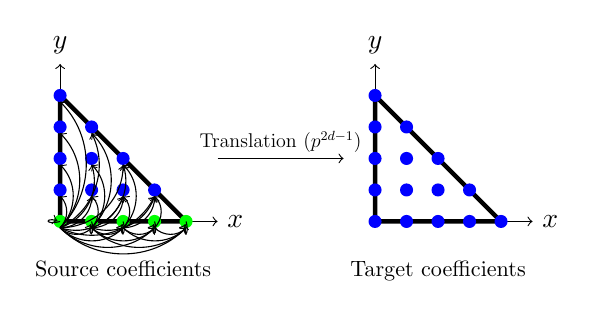
\begin{tikzpicture}[scale=0.4]
\draw[->] (0,0)--(5,0) node[right]{$x$};
\draw[->] (0,0)--(0,5) node[above]{$y$};
\draw[ultra thick] (0,0) node[anchor=north]{}
  -- (4,0) node[anchor=north]{}
  -- (0,4) node[anchor=south]{}
  -- cycle;
  
\foreach \Point in { (0, 0), (1.0, 0), (2.0, 0), (3.0, 0), (4.0, 0)}{
    \draw \Point node[anchor=center,fill=green,circle,scale=0.5] {};
}

\foreach \Point in { (0.0, 1.0), (0.0, 2.0), (0.0, 3.0), (0.0, 4.0), (1.0, 1.0), (1.0, 2.0), (1.0, 3.0), (2.0, 1.0), (2.0, 2.0), (3.0, 1.0) }{
    \draw \Point node[anchor=center,fill=blue,circle,scale=0.5] {};
}

%\draw[->, thick] (-0.2,0.2) to node[right] {} (-0.2, 0.2);
\path (0, 0) edge [loop left] node {} (0, 0);
\draw[->] (0,-0.2) to [bend right=45] node[right] {} (1,-0.2);
\draw[->] (0,-0.2) to [bend right=45] node[right] {} (2,-0.2);
\draw[->] (0,-0.2) to [bend right=45] node[right] {} (3,-0.2);
\draw[->] (0,-0.2) to [bend right=45] node[right] {} (4,-0.2);
\draw[->] (0,-0.2) to [bend right=45] node[right] {} (0,0.8);
\draw[->] (0,-0.2) to [bend right=45] node[right] {} (1,0.8);
\draw[->] (0,-0.2) to [bend right=45] node[right] {} (2,0.8);
\draw[->] (0,-0.2) to [bend right=45] node[right] {} (3,0.8);
\draw[->] (0,-0.2) to [bend right=45] node[right] {} (0,1.8);
\draw[->] (0,-0.2) to [bend right=45] node[right] {} (1,1.8);
\draw[->] (0,-0.2) to [bend right=45] node[right] {} (2,1.8);
\draw[->] (0,-0.2) to [bend right=45] node[right] {} (0,2.8);
\draw[->] (0,-0.2) to [bend right=45] node[right] {} (1,2.8);
\draw[->] (0,-0.2) to [bend right=45] node[right] {} (0,3.8);

\path (1, 0) edge [loop below] node {} (1, 0);
\draw[->] (1,-0.2) to [bend right=45] node[right] {} (2,-0.2);
\draw[->] (1,-0.2) to [bend right=45] node[right] {} (3,-0.2);
\draw[->] (1,-0.2) to [bend right=45] node[right] {} (4,-0.2);
\draw[->] (1,-0.2) to [bend right=45] node[right] {} (1,0.8);
\draw[->] (1,-0.2) to [bend right=45] node[right] {} (2,0.8);
\draw[->] (1,-0.2) to [bend right=45] node[right] {} (3,0.8);
\draw[->] (1,-0.2) to [bend right=45] node[right] {} (1,1.8);
\draw[->] (1,-0.2) to [bend right=45] node[right] {} (2,1.8);
\draw[->] (1,-0.2) to [bend right=45] node[right] {} (1,2.8);

\path (2, 0) edge [loop below] node {} (2, 0);
\draw[->] (2,-0.2) to [bend right=45] node[right] {} (3,-0.2);
\draw[->] (2,-0.2) to [bend right=45] node[right] {} (4,-0.2);
\draw[->] (2,-0.2) to [bend right=45] node[right] {} (2,0.8);
\draw[->] (2,-0.2) to [bend right=45] node[right] {} (3,0.8);
\draw[->] (2,-0.2) to [bend right=45] node[right] {} (2,1.8);
\node[below,scale=0.8] at (2,-1) {Source coefficients};

\path (3, 0) edge [loop below] node {} (3, 0);
\draw[->] (3,-0.2) to [bend right=45] node[right] {} (4,-0.2);
\draw[->] (3,-0.2) to [bend right=45] node[right] {} (3,0.8);

\path (4, 0) edge [loop below] node {} (4, 0);

\draw[->] (5, 2)-- node[above,scale=0.6]{\large Translation ($p^{2d-1}$)} (9, 2);
\draw[->] (10,0)--(15,0) node[right]{$x$};
\draw[->] (10,0)--(10,5) node[above]{$y$};
\draw[ultra thick] (10,0) node[anchor=north]{}
  -- (14,0) node[anchor=north]{}
  -- (10,4) node[anchor=south]{}
  -- cycle;
  
\foreach \Point in { (10, 0), (11.0, 0), (12.0, 0), (13.0, 0), (14.0, 0)}{
    \draw \Point node[anchor=center,fill=blue,circle,scale=0.5] {};
}

\foreach \Point in { (10.0, 1.0), (10.0, 2.0), (10.0, 3.0), (10.0, 4.0), (11.0, 1.0), (11.0, 2.0), (11.0, 3.0), (12.0, 1.0), (12.0, 2.0), (13.0, 1.0) }{
    \draw \Point node[anchor=center,fill=blue,circle,scale=0.5] {};
}

\node[below,scale=0.8] at (12,-1) {Target coefficients};
\end{tikzpicture}
\end{center}
\begin{center}
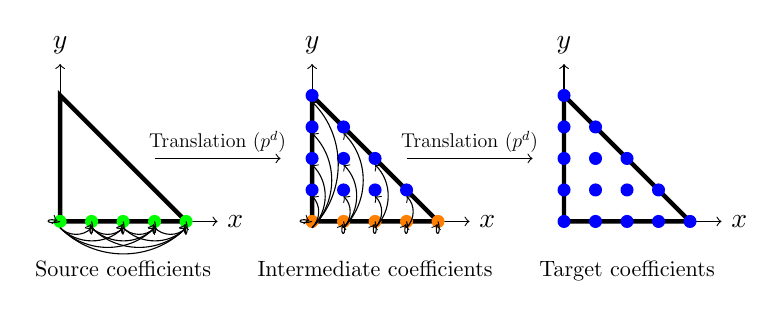
\begin{tikzpicture}[scale=0.4]
\draw[->] (0,0)--(5,0) node[right]{$x$};
\draw[->] (0,0)--(0,5) node[above]{$y$};
\draw[ultra thick] (0,0) node[anchor=north]{}
  -- (4,0) node[anchor=north]{}
  -- (0,4) node[anchor=south]{}
  -- cycle;
  
\foreach \Point in { (0, 0), (1.0, 0), (2.0, 0), (3.0, 0), (4.0, 0)}{
    \draw \Point node[anchor=center,fill=green,circle,scale=0.5] {};
}


%\draw[->, thick] (-0.2,0.2) to node[right] {} (-0.2, 0.2);
\path (0, 0) edge [loop left] node {} (0, 0);
\path (1, 0) edge [loop below] node {} (1, 0);
\path (2, 0) edge [loop below] node {} (2, 0);
\path (3, 0) edge [loop below] node {} (3, 0);
\path (4, 0) edge [loop below] node {} (4, 0);
\draw[->] (0,-0.2) to [bend right=45] node[right] {} (1,-0.2);
\draw[->] (0,-0.2) to [bend right=45] node[right] {} (2,-0.2);
\draw[->] (0,-0.2) to [bend right=45] node[right] {} (3,-0.2);
\draw[->] (0,-0.2) to [bend right=45] node[right] {} (4,-0.2);
\draw[->] (1,-0.2) to [bend right=45] node[right] {} (2,-0.2);
\draw[->] (1,-0.2) to [bend right=45] node[right] {} (3,-0.2);
\draw[->] (1,-0.2) to [bend right=45] node[right] {} (4,-0.2);
\draw[->] (2,-0.2) to [bend right=45] node[right] {} (3,-0.2);
\draw[->] (2,-0.2) to [bend right=45] node[right] {} (4,-0.2);
\draw[->] (3,-0.2) to [bend right=45] node[right] {} (4,-0.2);

\node[below,scale=0.8] at (2,-1) {Source coefficients};
\draw[->] (3, 2)-- node[above,scale=0.6]{\large Translation ($p^{d}$)} (7, 2);

\draw[->] (8,0)--(13,0) node[right]{$x$};
\draw[->] (8,0)--(8,5) node[above]{$y$};
\draw[ultra thick] (8,0) node[anchor=north]{}
  -- (12,0) node[anchor=north]{}
  -- (8,4) node[anchor=south]{}
  -- cycle;
  
\foreach \Point in { (8, 0), (9.0, 0), (10.0, 0), (11.0, 0), (12.0, 0)}{
    \draw \Point node[anchor=center,fill=orange,circle,scale=0.5] {};
}

\foreach \Point in { (8.0, 1.0), (8.0, 2.0), (8.0, 3.0), (8.0, 4.0), (9.0, 1.0), (9.0, 2.0), (9.0, 3.0), (10.0, 1.0), (10.0, 2.0), (11.0, 1.0) }{
    \draw \Point node[anchor=center,fill=blue,circle,scale=0.5] {};
}

\path (8, 0) edge [loop left] node {} (8, 0);
\path (9, 0) edge [loop below] node {} (9, 0);
\path (10, 0) edge [loop below] node {} (10, 0);
\path (11, 0) edge [loop below] node {} (11, 0);
\path (12, 0) edge [loop below] node {} (12, 0);
\draw[->] (8,-0.2) to [bend right=45] node[right] {} (8,0.8);
\draw[->] (8,-0.2) to [bend right=45] node[right] {} (8,1.8);
\draw[->] (8,-0.2) to [bend right=45] node[right] {} (8,2.8);
\draw[->] (8,-0.2) to [bend right=45] node[right] {} (8,3.8);
\draw[->] (9,-0.2) to [bend right=45] node[right] {} (9,0.8);
\draw[->] (9,-0.2) to [bend right=45] node[right] {} (9,1.8);
\draw[->] (9,-0.2) to [bend right=45] node[right] {} (9,2.8);
\draw[->] (10,-0.2) to [bend right=45] node[right] {} (10,0.8);
\draw[->] (10,-0.2) to [bend right=45] node[right] {} (10,1.8);
\draw[->] (11,-0.2) to [bend right=45] node[right] {} (11,0.8);

\node[below,scale=0.8] at (10,-1) {Intermediate coefficients};
\draw[->] (11, 2)-- node[above,scale=0.6]{\large Translation ($p^{d}$)} (15, 2);
\draw[->] (16,0)--(21,0) node[right]{$x$};
\draw[->] (16,0)--(16,5) node[above]{$y$};
\draw[ultra thick] (16,0) node[anchor=north]{}
  -- (20,0) node[anchor=north]{}
  -- (16,4) node[anchor=south]{}
  -- cycle;
  
\foreach \Point in { (16, 0), (17.0, 0), (18.0, 0), (19.0, 0), (20.0, 0)}{
    \draw \Point node[anchor=center,fill=blue,circle,scale=0.5] {};
}

\foreach \Point in { (16.0, 1.0), (16.0, 2.0), (16.0, 3.0), (16.0, 4.0), (17.0, 1.0), (17.0, 2.0), (17.0, 3.0), (18.0, 1.0), (18.0, 2.0), (19.0, 1.0) }{
    \draw \Point node[anchor=center,fill=blue,circle,scale=0.5] {};
}

\node[below,scale=0.8] at (18,-1) {Target coefficients};

\end{tikzpicture}
\end{center}

Note: For local to local translation, reverse all arrows.

\end{frame}
\begin{frame}[fragile]{Faster Compressed Multipole Translation}
\begin{center}
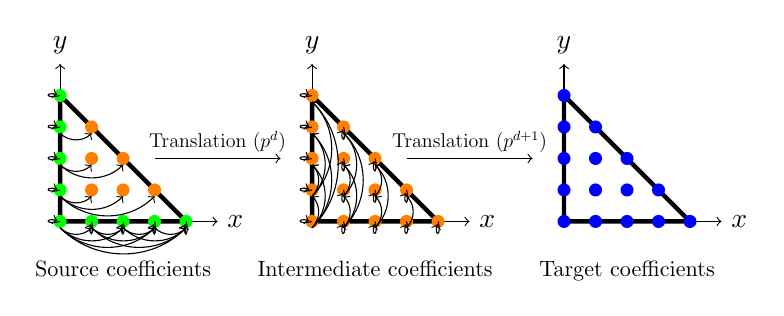
\begin{tikzpicture}[scale=0.4]
\draw[->] (0,0)--(5,0) node[right]{$x$};
\draw[->] (0,0)--(0,5) node[above]{$y$};
\draw[ultra thick] (0,0) node[anchor=north]{}
  -- (4,0) node[anchor=north]{}
  -- (0,4) node[anchor=south]{}
  -- cycle;
  
\foreach \Point in { (0, 0), (1.0, 0), (2.0, 0), (3.0, 0), (4.0, 0), (0, 1.0), (0, 2.0), (0, 3.0), (0, 4.0)}{
    \draw \Point node[anchor=center,fill=green,circle,scale=0.5] {};
}
\foreach \Point in { (1.0, 1.0), (1.0, 2.0), (1.0, 3.0), (2.0, 1.0), (2.0, 2.0), (3.0, 1.0) }{
    \draw \Point node[anchor=center,fill=orange,circle,scale=0.5] {};
}


%\draw[->, thick] (-0.2,0.2) to node[right] {} (-0.2, 0.2);
\path (0, 0) edge [loop left] node {} (0, 0);
\path (1, 0) edge [loop below] node {} (1, 0);
\path (2, 0) edge [loop below] node {} (2, 0);
\path (3, 0) edge [loop below] node {} (3, 0);
\path (4, 0) edge [loop below] node {} (4, 0);
\path (0, 1) edge [loop left] node {} (0, 1);
\path (0, 2) edge [loop left] node {} (0, 2);
\path (0, 3) edge [loop left] node {} (0, 3);
\path (0, 4) edge [loop left] node {} (0, 4);
\draw[->] (0,-0.2) to [bend right=45] node[right] {} (1,-0.2);
\draw[->] (0,-0.2) to [bend right=45] node[right] {} (2,-0.2);
\draw[->] (0,-0.2) to [bend right=45] node[right] {} (3,-0.2);
\draw[->] (0,-0.2) to [bend right=45] node[right] {} (4,-0.2);
\draw[->] (1,-0.2) to [bend right=45] node[right] {} (2,-0.2);
\draw[->] (1,-0.2) to [bend right=45] node[right] {} (3,-0.2);
\draw[->] (1,-0.2) to [bend right=45] node[right] {} (4,-0.2);
\draw[->] (2,-0.2) to [bend right=45] node[right] {} (3,-0.2);
\draw[->] (2,-0.2) to [bend right=45] node[right] {} (4,-0.2);
\draw[->] (3,-0.2) to [bend right=45] node[right] {} (4,-0.2);

\draw[->] (0,0.8) to [bend right=45] node[right] {} (1,0.8);
\draw[->] (0,0.8) to [bend right=45] node[right] {} (2,0.8);
\draw[->] (0,0.8) to [bend right=45] node[right] {} (3,0.8);

\draw[->] (0,1.8) to [bend right=45] node[right] {} (1,1.8);
\draw[->] (0,1.8) to [bend right=45] node[right] {} (2,1.8);
\draw[->] (0,2.8) to [bend right=45] node[right] {} (1,2.8);
\node[below,scale=0.8] at (2,-1) {Source coefficients};
\draw[->] (3, 2)-- node[above,scale=0.6]{\large Translation ($p^{d}$)} (7, 2);

\draw[->] (8,0)--(13,0) node[right]{$x$};
\draw[->] (8,0)--(8,5) node[above]{$y$};
\draw[ultra thick] (8,0) node[anchor=north]{}
  -- (12,0) node[anchor=north]{}
  -- (8,4) node[anchor=south]{}
  -- cycle;
  
\foreach \Point in { (8, 0), (9.0, 0), (10.0, 0), (11.0, 0), (12.0, 0)}{
    \draw \Point node[anchor=center,fill=orange,circle,scale=0.5] {};
}

\foreach \Point in { (8.0, 1.0), (8.0, 2.0), (8.0, 3.0), (8.0, 4.0), (9.0, 1.0), (9.0, 2.0), (9.0, 3.0), (10.0, 1.0), (10.0, 2.0), (11.0, 1.0) }{
    \draw \Point node[anchor=center,fill=orange,circle,scale=0.5] {};
}

\path (8, 0) edge [loop left] node {} (8, 0);
\path (8, 1) edge [loop left] node {} (8, 1);
\path (8, 2) edge [loop left] node {} (8, 2);
\path (8, 3) edge [loop left] node {} (8, 3);
\path (8, 4) edge [loop left] node {} (8, 4);
\path (9, 0) edge [loop below] node {} (9, 0);
\path (9, 1) edge [loop below] node {} (9, 1);
\path (9, 2) edge [loop below] node {} (9, 2);
\path (9, 3) edge [loop below] node {} (9, 3);
\path (10, 0) edge [loop below] node {} (10, 0);
\path (10, 1) edge [loop below] node {} (10, 1);
\path (10, 2) edge [loop below] node {} (10, 2);
\path (11, 0) edge [loop below] node {} (11, 0);
\path (11, 1) edge [loop below] node {} (11, 1);
\path (12, 0) edge [loop below] node {} (12, 0);
\draw[->] (8,-0.2) to [bend right=45] node[right] {} (8,0.8);
\draw[->] (8,-0.2) to [bend right=45] node[right] {} (8,1.8);
\draw[->] (8,-0.2) to [bend right=45] node[right] {} (8,2.8);
\draw[->] (8,-0.2) to [bend right=45] node[right] {} (8,3.8);
\draw[->] (9,-0.2) to [bend right=45] node[right] {} (9,0.8);
\draw[->] (9,-0.2) to [bend right=45] node[right] {} (9,1.8);
\draw[->] (9,-0.2) to [bend right=45] node[right] {} (9,2.8);
\draw[->] (10,-0.2) to [bend right=45] node[right] {} (10,0.8);
\draw[->] (10,-0.2) to [bend right=45] node[right] {} (10,1.8);
\draw[->] (11,-0.2) to [bend right=45] node[right] {} (11,0.8);

\draw[->] (8,0.8) to [bend right=45] node[right] {} (8,1.8);
\draw[->] (8,0.8) to [bend right=45] node[right] {} (8,2.8);
\draw[->] (8,0.8) to [bend right=45] node[right] {} (8,3.8);
\draw[->] (9,0.8) to [bend right=45] node[right] {} (9,1.8);
\draw[->] (9,0.8) to [bend right=45] node[right] {} (9,2.8);
\draw[->] (10,0.8) to [bend right=45] node[right] {} (10,1.8);
\node[below,scale=0.8] at (10,-1) {Intermediate coefficients};
\draw[->] (11, 2)-- node[above,scale=0.6]{\large Translation ($p^{d+1}$)} (15, 2);
\draw[->] (16,0)--(21,0) node[right]{$x$};
\draw[->] (16,0)--(16,5) node[above]{$y$};
\draw[ultra thick] (16,0) node[anchor=north]{}
  -- (20,0) node[anchor=north]{}
  -- (16,4) node[anchor=south]{}
  -- cycle;
  
\foreach \Point in { (16, 0), (17.0, 0), (18.0, 0), (19.0, 0), (20.0, 0)}{
    \draw \Point node[anchor=center,fill=blue,circle,scale=0.5] {};
}

\foreach \Point in { (16.0, 1.0), (16.0, 2.0), (16.0, 3.0), (16.0, 4.0), (17.0, 1.0), (17.0, 2.0), (17.0, 3.0), (18.0, 1.0), (18.0, 2.0), (19.0, 1.0) }{
    \draw \Point node[anchor=center,fill=blue,circle,scale=0.5] {};
}

\node[below,scale=0.8] at (18,-1) {Target coefficients};

\end{tikzpicture}
\end{center}
\pause
Divide the problem into 2 subproblems to keep the cost down to $\mathcal{O}(p^d)$.
\begin{center}
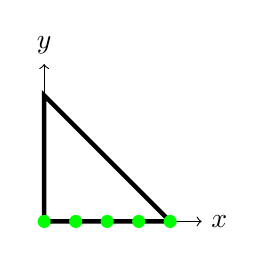
\begin{tikzpicture}[scale=0.4]
\draw[->] (0,0)--(5,0) node[right]{$x$};
\draw[->] (0,0)--(0,5) node[above]{$y$};
\draw[ultra thick] (0,0) node[anchor=north]{}
  -- (4,0) node[anchor=north]{}
  -- (0,4) node[anchor=south]{}
  -- cycle;
  
\foreach \Point in { (0, 0), (1.0, 0), (2.0, 0), (3.0, 0), (4.0, 0)}{
    \draw \Point node[anchor=center,fill=green,circle,scale=0.5] {};
}
\end{tikzpicture}
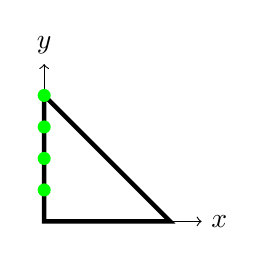
\begin{tikzpicture}[scale=0.4]
\draw[->] (0,0)--(5,0) node[right]{$x$};
\draw[->] (0,0)--(0,5) node[above]{$y$};
\draw[ultra thick] (0,0) node[anchor=north]{}
  -- (4,0) node[anchor=north]{}
  -- (0,4) node[anchor=south]{}
  -- cycle;
  
\foreach \Point in { (0, 1.0), (0, 2.0), (0, 3.0), (0, 4.0)}{
    \draw \Point node[anchor=center,fill=green,circle,scale=0.5] {};
}
\end{tikzpicture}
\end{center}


\end{frame}

\begin{frame}[fragile]{Compressed Multipole to Local Translation}
From multipole expansion, we get,
\[
 \psi(\b t, \b s) = \sum_{|m| \le k} \underbrace{\frac{D_{\b s}^m \psi(\b t, \b s)\Bigr|_{\b s = \b c}}{m!}}_{\text{depends on tgt/ctr}} \underbrace{(\b s - \b c)^m}_{\text{depends on src/ctr}}
\]
To translate this multipole expansion to a local expansion, we need to get
the derivatives of the above expression and evalaute at new center.

Cost: $\mathcal{O}(p^{2d-2})$.

\end{frame}

\begin{frame}[fragile]{Compressed Multipole to Local Translation}

Multipole to local translation matrix is a block Toeplitz matrix of smaller Toeplitz matrices.

\begin{center}
\begin{figure}
\includegraphics[scale=0.3]{figures/m2l_imshow.pdf}
\pause
\includegraphics[scale=0.3]{figures/m2l_imshow_2.pdf}
\end{figure}
\end{center}

Use an FFT to do the translation similar to Greengard (1988).

Cost depends on number of dummy rows:
 \begin{itemize}
     \item $\mathcal{O}(p^{d-1}\log(p))$ for elliptic PDEs
     \item $\mathcal{O}(p^{d}\log(p))$ for other PDEs
 \end{itemize}
\end{frame}

\begin{frame}[fragile]{Time complexities}

\renewcommand{\arraystretch}{2} 
 \begin{table}[]
 \scriptsize
 \begin{tabular}{|m{12em}|c|c|c|c|c|c|c|}
 \hline                          & P2L/M2P      & P2M/L2P   & M2M          & M2L            & L2L      \\ \hline
 Taylor Series                   & \color{NavyBlue} $\b  p^3$    &\color{NavyBlue} $\b p^3$ &\color{NavyBlue} $\b p^{6}$      &\color{NavyBlue} $\b p^{6}$        &\color{NavyBlue} $\b p^{6}$   \\ \hline
 Improved Taylor Series          & \color{NavyBlue} $\b  p^3$    &\color{NavyBlue} $\b p^3$ &\color{NavyBlue} $\b p^{4}$      &\color{NavyBlue} $\b p^{3} \log( \b p)$        &\color{NavyBlue} $\b p^{4}$   \\ \hline
     Compressed Taylor Series without fast derivatives          &\color{NavyBlue} $\b p^3$    &\color{NavyBlue} $\b p^3$ &\color{NavyBlue} $\b p^{3}$      &\color{Green} $\b p^{2} \log(\b p)$ & \color{NavyBlue}$\b p^{3}$   \\ \hline
 \textbf{Compressed Taylor Series with fast derivatives}
                                 &\color{Green} $\b p^{2}$  & \color{NavyBlue} $\b p^3$ &\color{NavyBlue} $\b p^{3}$      &\color{Green} $\b p^2 \log(\b p)$   &\color{NavyBlue} $\b p^{3}$   \\ \hline
 Spherical Harmonic Series       &\color{Green} $\b p^2$    &\color{Green} $\b p^2$ &\color{Green} $\b p^2\log(\b p)$ &\color{Green} $\b p^2\log(\b p)$   &\color{Green} $\b p^2\log(\b p)$   \\ \hline
 \end{tabular}
   \caption{Time complexities for expansions, translations and evaluations} \label{tab:compressed}
 \end{table}
All operations are exact except for M2M in Compressed Taylor and M2L operations with FFT.

\end{frame}

\begin{frame}[fragile]{Code generation}
 With Compressed Taylor generating code for Stokes
 \begin{align*} \mu \nabla^2 \mathbf{u} -\boldsymbol{\nabla}p + \mathbf{f} &= \boldsymbol{0} \\
 \boldsymbol{\nabla}\cdot\mathbf{u}&= 0 \end{align*}

 is done simply by giving the PDE as:
 
 \begin{minted}{python}
    w = make_pde_syms(ndims=3, neqs=4)
    mu = sym.Symbol("mu")
    u = w[:3]
    p = w[-1]
    pdes = PDE(mu * laplacian(u) - grad(p), div(u))
 \end{minted}
 which generates code for the expansion, translations and evaluations.

\end{frame}

\begin{frame}[fragile]{Code generation}
\begin{figure}
\includegraphics[scale=0.3]{figures/codegen-time-stokes-3d.pdf}
\includegraphics[scale=0.3]{figures/codegen-time-helmholtz-3d.pdf}
\includegraphics[scale=0.3]{figures/codegen-time-biharmonic-3d.pdf}
\includegraphics[scale=0.3]{figures/codegen-time-laplace-3d.pdf}
\end{figure}
\end{frame}
\begin{frame}[fragile]{Results - Error M2M}
\begin{figure}
\includegraphics[scale=0.3]{figures/accuracy-stokes-3d.pdf}
\includegraphics[scale=0.3]{figures/accuracy-helmholtz-3d.pdf}
\includegraphics[scale=0.3]{figures/accuracy-biharmonic-3d.pdf}
\includegraphics[scale=0.3]{figures/accuracy-laplace-3d.pdf}
\end{figure}
\end{frame}

\begin{frame}[fragile]{Results - FLOP count}
\begin{figure}
\includegraphics[scale=0.3]{figures/flops-laplace-M2L-3d.pdf}
\includegraphics[scale=0.3]{figures/flops-laplace-M2M-3d.pdf}
\includegraphics[scale=0.3]{figures/flops-laplace-M2P-3d.pdf}
\includegraphics[scale=0.3]{figures/flops-laplace-P2M-3d.pdf}
\end{figure}
\end{frame}

\begin{frame}[fragile]{Summary}
\begin{itemize}
 \item Kernel-generic method for elliptic constant coefficient linear PDEs
     with non-oscillatory kernels (for now).
 \item Only needs the PDE and the Green's function for the PDE.
 \item Asymptotically better than full Taylor Series in
    \begin{itemize}
     \item Number of FLOPs
     \item Storage
    \end{itemize}
  \item Next goal: A fast Stokes solver on a GPU.
\end{itemize}

Ackowledgements: 
    \begin{itemize}
        \item NSF grants 19-11019 and 16-54756
        \item SIAM travel grant
    \end{itemize}
\end{frame}

\end{document}

